\begin{table*}[t]
\centering
\caption{Fresh five-run post-processing measurements (13--14 October 2026) for 31 attempted upstream-generated configurations; 29 produced optimizer inputs. Comp. is the automaton after reset completion. $L$ counts graph-reachable locations, $E$ counts transitions from those locations, and $C$ counts active clocks used in guards or resets; $n_f$ is the formula-clock-key count. Opt. and Exp. give reachable $L/E/C$, changed optimization rounds, stage medians, invariant-bearing locations, and diagonal-guard occurrences. R7 and R8 time out upstream, before the optimizer boundary.}
\label{tab:optimizer-benchmarks}
\scriptsize
\setlength{\tabcolsep}{3pt}
\begin{adjustbox}{max width=\textwidth}\begin{tabular}{@{}lccccccccc@{}}
\toprule
ID & Comp. $L/E/C$ & $n_f$ & Opt. $L/E/C$ & Rnds & Opt. (s) & Exp. $L/E/C$ & Inv. & Diag. & Exp. (s)\\
\midrule
F1 & 2/5/1 & 1 & 2/5/1 & 1 & $<0.01$ & 2/5/1 & 1 & 0 & $<0.01$\\
F2 & 2/5/1 & 1 & 1/1/0 & 1 & $<0.01$ & 1/1/0 & 0 & 0 & $<0.01$\\
F3 & 2/5/1 & 1 & 2/5/1 & 1 & $<0.01$ & 2/5/1 & 0 & 0 & $<0.01$\\
F3b & 1/1/0 & 1 & 1/1/0 & 0 & $<0.01$ & 1/1/0 & 0 & 0 & $<0.01$\\
F4 & 2/5/1 & 1 & 2/5/1 & 1 & $<0.01$ & 2/5/1 & 1 & 0 & $<0.01$\\
F5 & 7/38/1 & 1 & 7/25/1 & 1 & $<0.01$ & 7/25/1 & 0 & 0 & 0.01\\
F6 & 7/38/1 & 1 & 7/25/1 & 1 & $<0.01$ & 7/25/1 & 0 & 0 & $<0.01$\\
F7 & 2/4/1 & 1 & 2/4/1 & 1 & $<0.01$ & 2/4/1 & 1 & 0 & $<0.01$\\
F8 & 2/4/0 & 0 & 2/4/0 & 1 & $<0.01$ & 2/4/0 & 0 & 0 & $<0.01$\\
F9 & 4/9/2 & 2 & 4/9/2 & 1 & $<0.01$ & 4/9/2 & 2 & 0 & $<0.01$\\
F10 & 5/13/3 & 3 & 5/13/3 & 1 & $<0.01$ & 5/13/3 & 2 & 0 & $<0.01$\\
F11 & 4/7/2 & 2 & 3/4/1 & 2 & $<0.01$ & 3/4/1 & 1 & 0 & $<0.01$\\
F12 & 3/9/2 & 2 & 2/5/2 & 2 & $<0.01$ & 2/5/2 & 1 & 0 & $<0.01$\\
F13 & 3/6/2 & 2 & 2/3/1 & 2 & $<0.01$ & 2/3/1 & 1 & 0 & $<0.01$\\
F14 & 6/23/2 & 2 & 6/17/2 & 1 & $<0.01$ & 6/19/2 & 4 & 2 & $<0.01$\\
R1 & 2/5/1 & 1 & 2/5/1 & 1 & $<0.01$ & 2/5/1 & 1 & 0 & $<0.01$\\
R2 & 4/25/2 & 2 & 4/16/2 & 2 & $<0.01$ & 4/19/2 & 3 & 2 & $<0.01$\\
R3 & 8/125/3 & 3 & 8/44/3 & 3 & 0.01 & 8/67/3 & 7 & 30 & 0.01\\
R4 & 16/625/4 & 4 & 16/112/4 & 4 & 0.06 & 16/217/4 & 15 & 192 & 0.16\\
R5 & 32/3125/5 & 5 & 32/272/5 & 5 & 0.94 & 32/651/5 & 31 & 880 & 1.45\\
R6 & 64/15625/6 & 6 & 64/640/6 & 6 & 17.81 & 64/1837/6 & 63 & 3360 & 10.67\\
R7 & -- & -- & -- & -- & -- & -- & -- & -- & --\\
R8 & -- & -- & -- & -- & -- & -- & -- & -- & --\\
N1 & 3/5/1 & 1 & 3/5/1 & 1 & $<0.01$ & 3/5/1 & 1 & 0 & $<0.01$\\
N2 & 4/11/2 & 2 & 4/9/2 & 1 & $<0.01$ & 4/9/2 & 2 & 0 & $<0.01$\\
N3 & 5/21/3 & 3 & 5/16/3 & 1 & $<0.01$ & 5/16/3 & 3 & 0 & $<0.01$\\
N4 & 6/36/4 & 4 & 6/25/4 & 1 & $<0.01$ & 6/25/4 & 4 & 0 & 0.01\\
N5 & 7/57/5 & 5 & 7/36/5 & 1 & 0.01 & 7/36/5 & 5 & 0 & 0.02\\
N6 & 8/85/6 & 6 & 8/49/6 & 1 & 0.03 & 8/49/6 & 6 & 0 & 0.06\\
N7 & 9/121/7 & 7 & 9/64/7 & 1 & 0.10 & 9/64/7 & 7 & 0 & 0.23\\
N8 & 10/166/8 & 8 & 10/81/8 & 1 & 0.33 & 10/81/8 & 8 & 0 & 0.70\\
\bottomrule
\end{tabular}\end{adjustbox}
\end{table*}




\begin{figure*}[t]
\centering
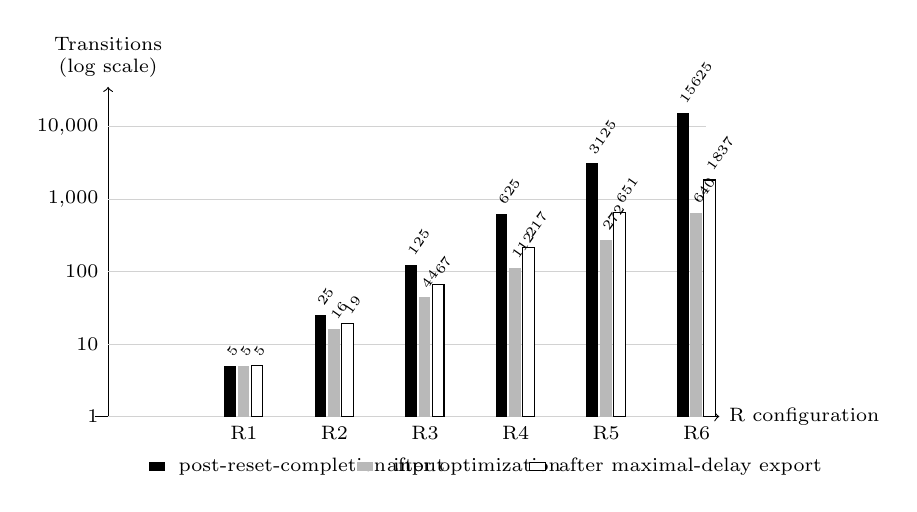
\begin{tikzpicture}[x=1.15cm,y=0.92cm,font=\scriptsize]
  % Vertical positions encode log10(edge count); the labelled y ticks are
  % 1, 10, 100, 1,000, and 10,000 transitions.
  \draw[->] (0.1,0) -- (7.0,0) node[right] {R configuration};
  \draw[->] (0.25,0) -- (0.25,4.55) node[above,align=center]
    {Transitions\\(log scale)};
  \foreach \y/\lab in {0/1,1/10,2/100,3/1{,}000,4/10{,}000} {
    \draw[gray!35] (0.25,\y) -- (6.85,\y);
    \node[left] at (0.25,\y) {\lab};
  }
  % Bars use log10(value) as height. Values above bars are exact counts.
  \foreach \x/\vin/\hin/\vopt/\hopt/\vexp/\hexp in {
    1/5/0.699/5/0.699/5/0.699,
    2/25/1.398/16/1.204/19/1.279,
    3/125/2.097/44/1.643/67/1.826,
    4/625/2.796/112/2.049/217/2.336,
    5/3125/3.494/272/2.435/651/2.814,
    6/15625/4.194/640/2.806/1837/3.264
  } {
    \pgfmathsetmacro{\xc}{\x+0.75}
    \pgfmathsetmacro{\xa}{\xc-0.22}
    \pgfmathsetmacro{\xb}{\xc-0.07}
    \pgfmathsetmacro{\xd}{\xc+0.08}
    \fill[black] (\xa,0) rectangle +(0.13,\hin);
    \fill[gray!55] (\xb,0) rectangle +(0.13,\hopt);
    \fill[white] (\xd,0) rectangle +(0.13,\hexp);
    \draw (\xd,0) rectangle +(0.13,\hexp);
    \node[rotate=55,anchor=west,font=\tiny] at (\xa,\hin+0.04) {\vin};
    \node[rotate=55,anchor=west,font=\tiny] at (\xb,\hopt+0.04) {\vopt};
    \node[rotate=55,anchor=west,font=\tiny] at (\xd,\hexp+0.04) {\vexp};
    \node[below] at (\xc,0) {R\x};
  }
  \fill[black] (0.7,-0.75) rectangle +(0.18,0.12);
  \node[right] at (0.92,-0.69) {post-reset-completion input};
  \fill[gray!55] (3.0,-0.75) rectangle +(0.18,0.12);
  \node[right] at (3.22,-0.69) {after optimization};
  \fill[white] (4.9,-0.75) rectangle +(0.18,0.12);
  \draw (4.9,-0.75) rectangle +(0.18,0.12);
  \node[right] at (5.12,-0.69) {after maximal-delay export};
\end{tikzpicture}

\caption{Post-reset-completion input, optimized TBA, and maximal-delay
explicit export for R1--R6. The logarithmic vertical axis makes the R6
concentration visible. These are positive forms measured with Spot level \texttt{small} and the implementation before the speedups (R7 and R8 did not complete); the counts are five-run medians, and
Comp. (the post-reset-completion input) is the optimizer boundary, regardless of whether an upstream
Spot count happens to match it.}
\label{fig:R-transition-counts}
\end{figure*}

\subsection{Optimization effects on the generated group}
In R6, Spot emits 64 states and 15,625 cube-split transitions. The recorded
post-reset-completion optimizer input also has 64 locations and 15,625
transitions; the equality of these two edge counts is specific to R6, and the
Comp. column is the authoritative optimizer boundary. Six optimization
rounds reduce the transition relation to 640 edges and retain six clocks.
Export then produces 1,837 explicit edges, 63 invariant-bearing locations,
and 3,360 clock-difference guard occurrences; symbolic grouping represents
the output with 448 transitions. The larger explicit edge count results from
splitting disjunctive guards and adding entry conditions for invariant copies.
It measures the cost of the target representation, not a reversal of the
optimizer's reduction. In the fresh run, median optimizer and export times
are 17.807 s and 10.666 s, respectively; these are times of the build before the verified speedups of article Section~\ref{sec:speedups}, with which the optimization of the positive form of R6 takes 0.29~s. Figure~\ref{fig:R-transition-counts} shows the concentration on R6. The generated-group table separately reports the
stage after reset completion so that upstream processing is not folded into
these optimizer measurements.

The same distinction matters for the other generated inputs. For example,
F11 starts from its actual four-location, seven-transition, two-clock TBA
after reset completion; two rounds leave three locations and four
transitions and remove one clock. Two locations have the same loop and the
same exit on $p$ to the accepting location, except that the exit of the first
also carries $x\ge2$; the second is entered only when $x\ge2$ holds and $x$ is
not reset afterwards. They are merged because the guards are compared under
that entry invariant, which equality of guards cannot do. N8 spends most of its end-to-end time in Spot,
whereas its recorded optimizer and exporter stages take 0.33 s and 0.70 s.
These cases show that the optimizer's cost depends on its input relation and
that the upstream producer can dominate total tool time. They do not support
a general runtime or size bound. The runs of this subsection used the former default, Spot level \texttt{small}.
The tool's default is now the automatic mode of article Section~\ref{sec:spot-level};
with level \texttt{low} N8 (positive form) takes 11.6 s instead of 98.3 s, and
the total over the 29 completed configurations falls from 152 s to 58 s (one
run against the five-run medians); optimized sizes are identical except for F5
and F6 (25 to 27 symbolic transitions). The optimizer, the export and the
initial-value check were since made faster by verified rewritings
(article Section~\ref{sec:speedups}), so the timings of the table are those of the
earlier implementation.

